\documentclass{standalone}
\usepackage{tikz}
\usepackage{ctex,siunitx}
\setCJKmainfont{Noto Serif CJK SC}
\usepackage{tkz-euclide}
\usepackage{amsmath}
\usetikzlibrary{patterns, calc,3d}
\usetikzlibrary {decorations.pathmorphing,decorations.pathreplacing,decorations.shapes}
\begin{document}
\small
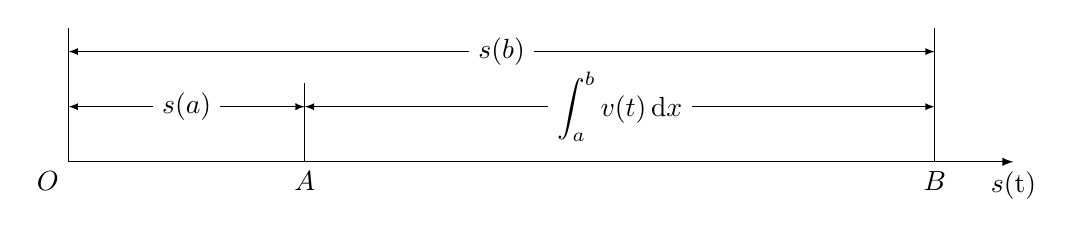
\begin{tikzpicture}[>=latex,scale=1.0]
  \draw[->](0,0)node[below left]{$O$}--(12,0)node[below]{$s$(\unit{t})};
  \draw[very thin](0,0)--(0,1.7)(3,0)node[below]{$A$}--(3,1)(11,0)node[below]{$B$}--(11,1.7);
  \draw[very thin,<->](3,0.7)--(11,0.7)node[midway,fill=white]{$\displaystyle \int_a^b v(t)\,\mathrm{d}x$};
  \draw[very thin,<->](0,0.7)--(3,0.7)node[midway,fill=white]{$s(a)$};
  \draw[very thin,<->](0,1.4)--(11,1.4)node[midway,fill=white]{$s(b)$};
\end{tikzpicture}
\end{document}